\begin{sepframe}{Composition}{Moving from \texttt{is-a} to \texttt{has-a}}
\end{sepframe}

\begin{frame}[fragile,c]
    \frametitle{Composition and inheritance}
    \framesubtitle{Map}

    \makebox[\linewidth]{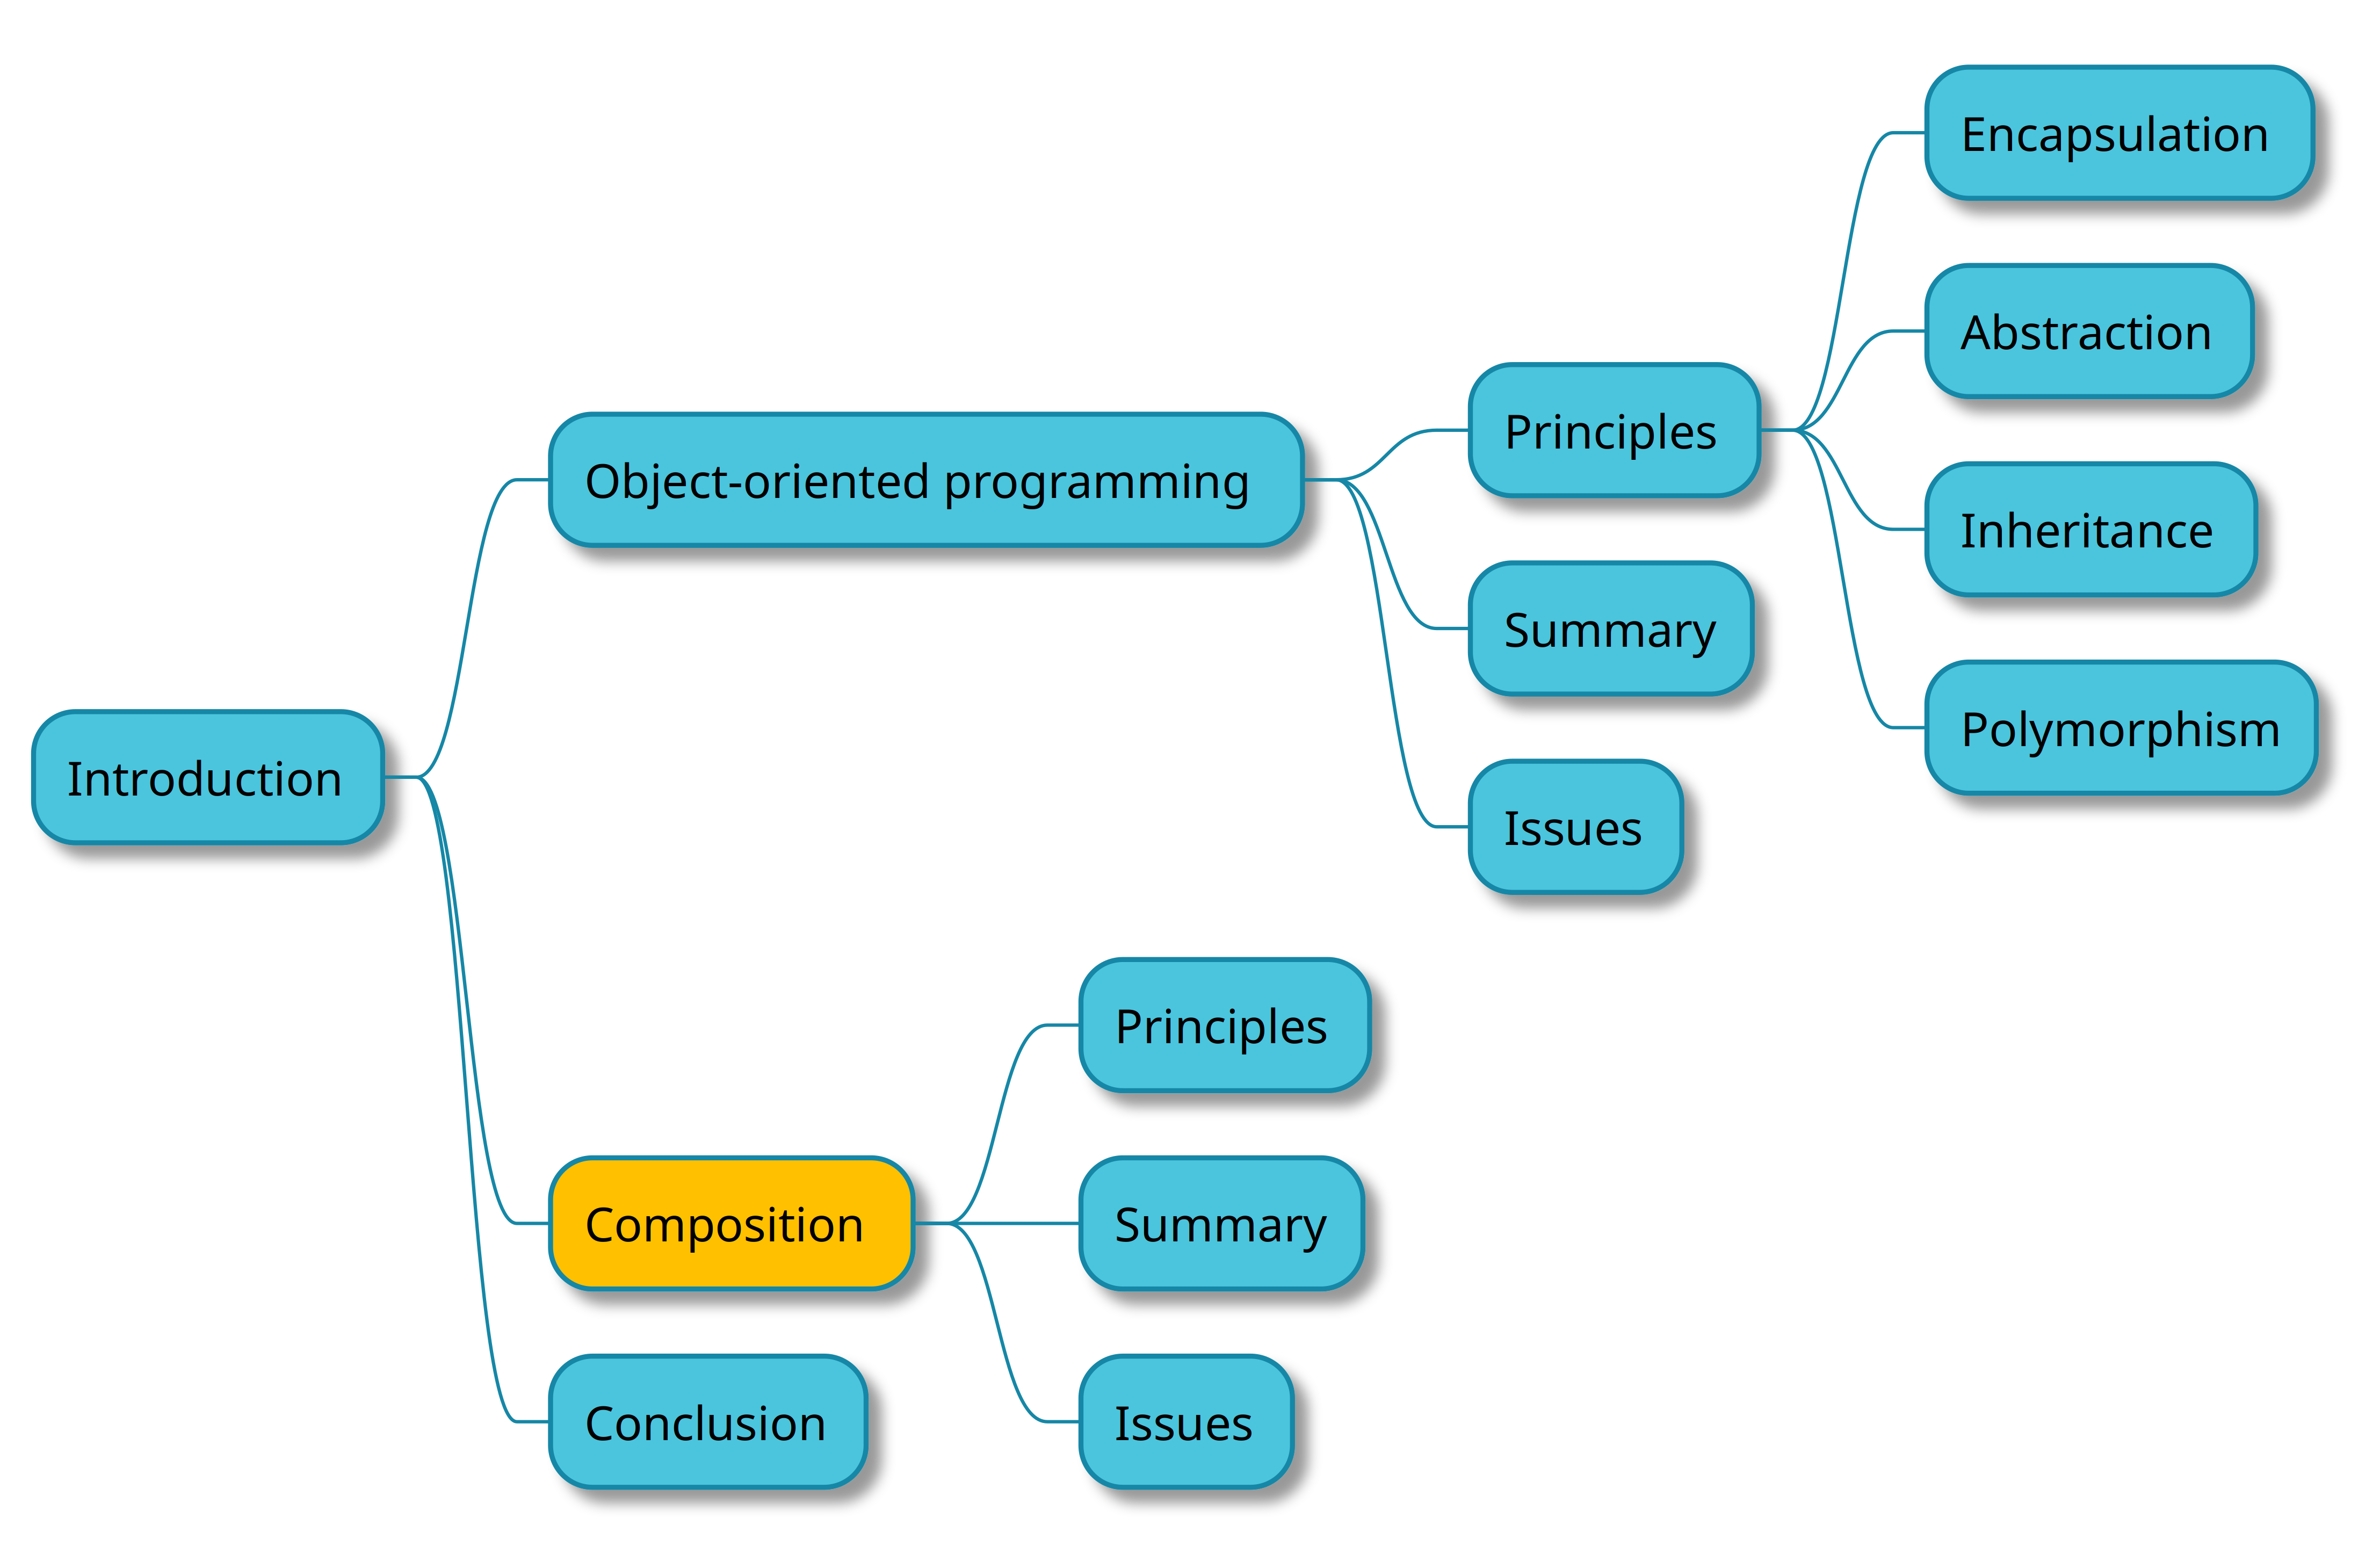
\includegraphics[width=\paperwidth]{src/session--composition-and-inheritance/resources/summary-composition-intro.png}}
\end{frame}

\begin{frame}
    \frametitle{Object-oriented programming with composition}
    \framesubtitle{Principles}

    \begin{itemize}[<+->]
        \item Encapsulation
        \item Abstraction
        \item \only<3-4>{Inheritance}\only<5->{\sout{Inheritance} \textbf{Composition}}
        \item Polymorphism
    \end{itemize}
\end{frame}

% Add slide here explaining what Composition is.

\begin{frame}
    \frametitle{Object-oriented programming with composition}
    \framesubtitle{The good things}

    \begin{itemize}[<+->]
        \item We use it every day,
        \item Natural and very simple to use.
    \end{itemize}
\end{frame}

\begin{frame}[fragile,c]
    \begin{lstlisting}
<?php

interface Ingredient {}

interface Pizza {
    public function getIngredients(): array;
}
    \end{lstlisting}
\end{frame}

\begin{frame}[fragile,c]
    \begin{lstlisting}
<?php

final class Margherita implements Pizza
{
    public function __construct(
        private Ingredient $tomato,
        private Ingredient $cheese
    ) {}

    public function getIngredients(): array
    {
        return [$this->tomato, $this->cheese];
    }
}
    \end{lstlisting}
\end{frame}

\begin{frame}[fragile,c]
    \begin{lstlisting}
<?php

final class Siciliana implements Pizza
{
    public function __construct(
        private Ingredient $tomato,
        private Ingredient $cheese
        private Ingredient $mushroom
    ) {}

    public function getIngredients(): array
    {
        return [$this->tomato, $this->cheese, $this->mushroom];
    }
}
    \end{lstlisting}
\end{frame}

\begin{frame}[fragile,c]
    \begin{lstlisting}
<?php

final class Regina implements Pizza
{
    public function __construct(
        private Ingredient $tomato,
        private Ingredient $cheese,
        private Ingredient $mushroom,
        private Ingredient $ham
    ) {}

    public function getIngredients(): array
    {
        return [$this->tomato, $this->cheese, $this->mushroom, $this->ham];
    }
}
    \end{lstlisting}
\end{frame}

\begin{frame}[fragile,c]
    \begin{lstlisting}
<?php

final class Parmigiana implements Pizza
{
    public function __construct(
        private Ingredient $tomato,
        private Ingredient $cheese,
        private Ingredient $mushroom,
        private Ingredient $aubergine
    ) {}

    public function getIngredients(): array
    {
        return [$this->tomato, $this->cheese, $this->mushroom, $this->aubergine];
    }
}
    \end{lstlisting}
\end{frame}

\begin{frame}[fragile,c]
    \begin{lstlisting}
<?php

final class Napoli implements Pizza
{
    public function __construct(
        private Ingredient $tomato,
        private Ingredient $cheese,
        private Ingredient $mushroom,
        private Ingredient $ham,
        private Ingredient $artichoke,
        private Ingredient $aubergine
    ) {}

    public function getIngredients(): array
    {
        return [
            $this->tomato,
            $this->cheese,
            $this->mushroom,
            $this->ham,
            $this->artichoke,
            $this->aubergine
        ];
    }
}
    \end{lstlisting}
\end{frame}

\begin{frame}[fragile,c]
    \begin{lstlisting}
<?php

$tomato = new Tomato;
$cheese = new Cheese;
$mushroom = new Mushroom;
$ham = new Ham;
$aubergine = new Aubergine;
$artichoke = new Artichoke;

$marguerita = new Margherita($tomato, $cheese);

$siciliana = new Siciliana($tomato, $cheese, $muschroom);

$regina = new Regina($tomato, $cheese, $mushroom, $ham);

$parmigiana = new Parmigiana($tomato, $cheese, $mushroom, $aubergine);

$napoli = new Napoli($tomato, $cheese, $mushroom, $ham, $aubergine, $artichoke);
    \end{lstlisting}
\end{frame}

\begin{frame}[fragile,c]
    \begin{center}
        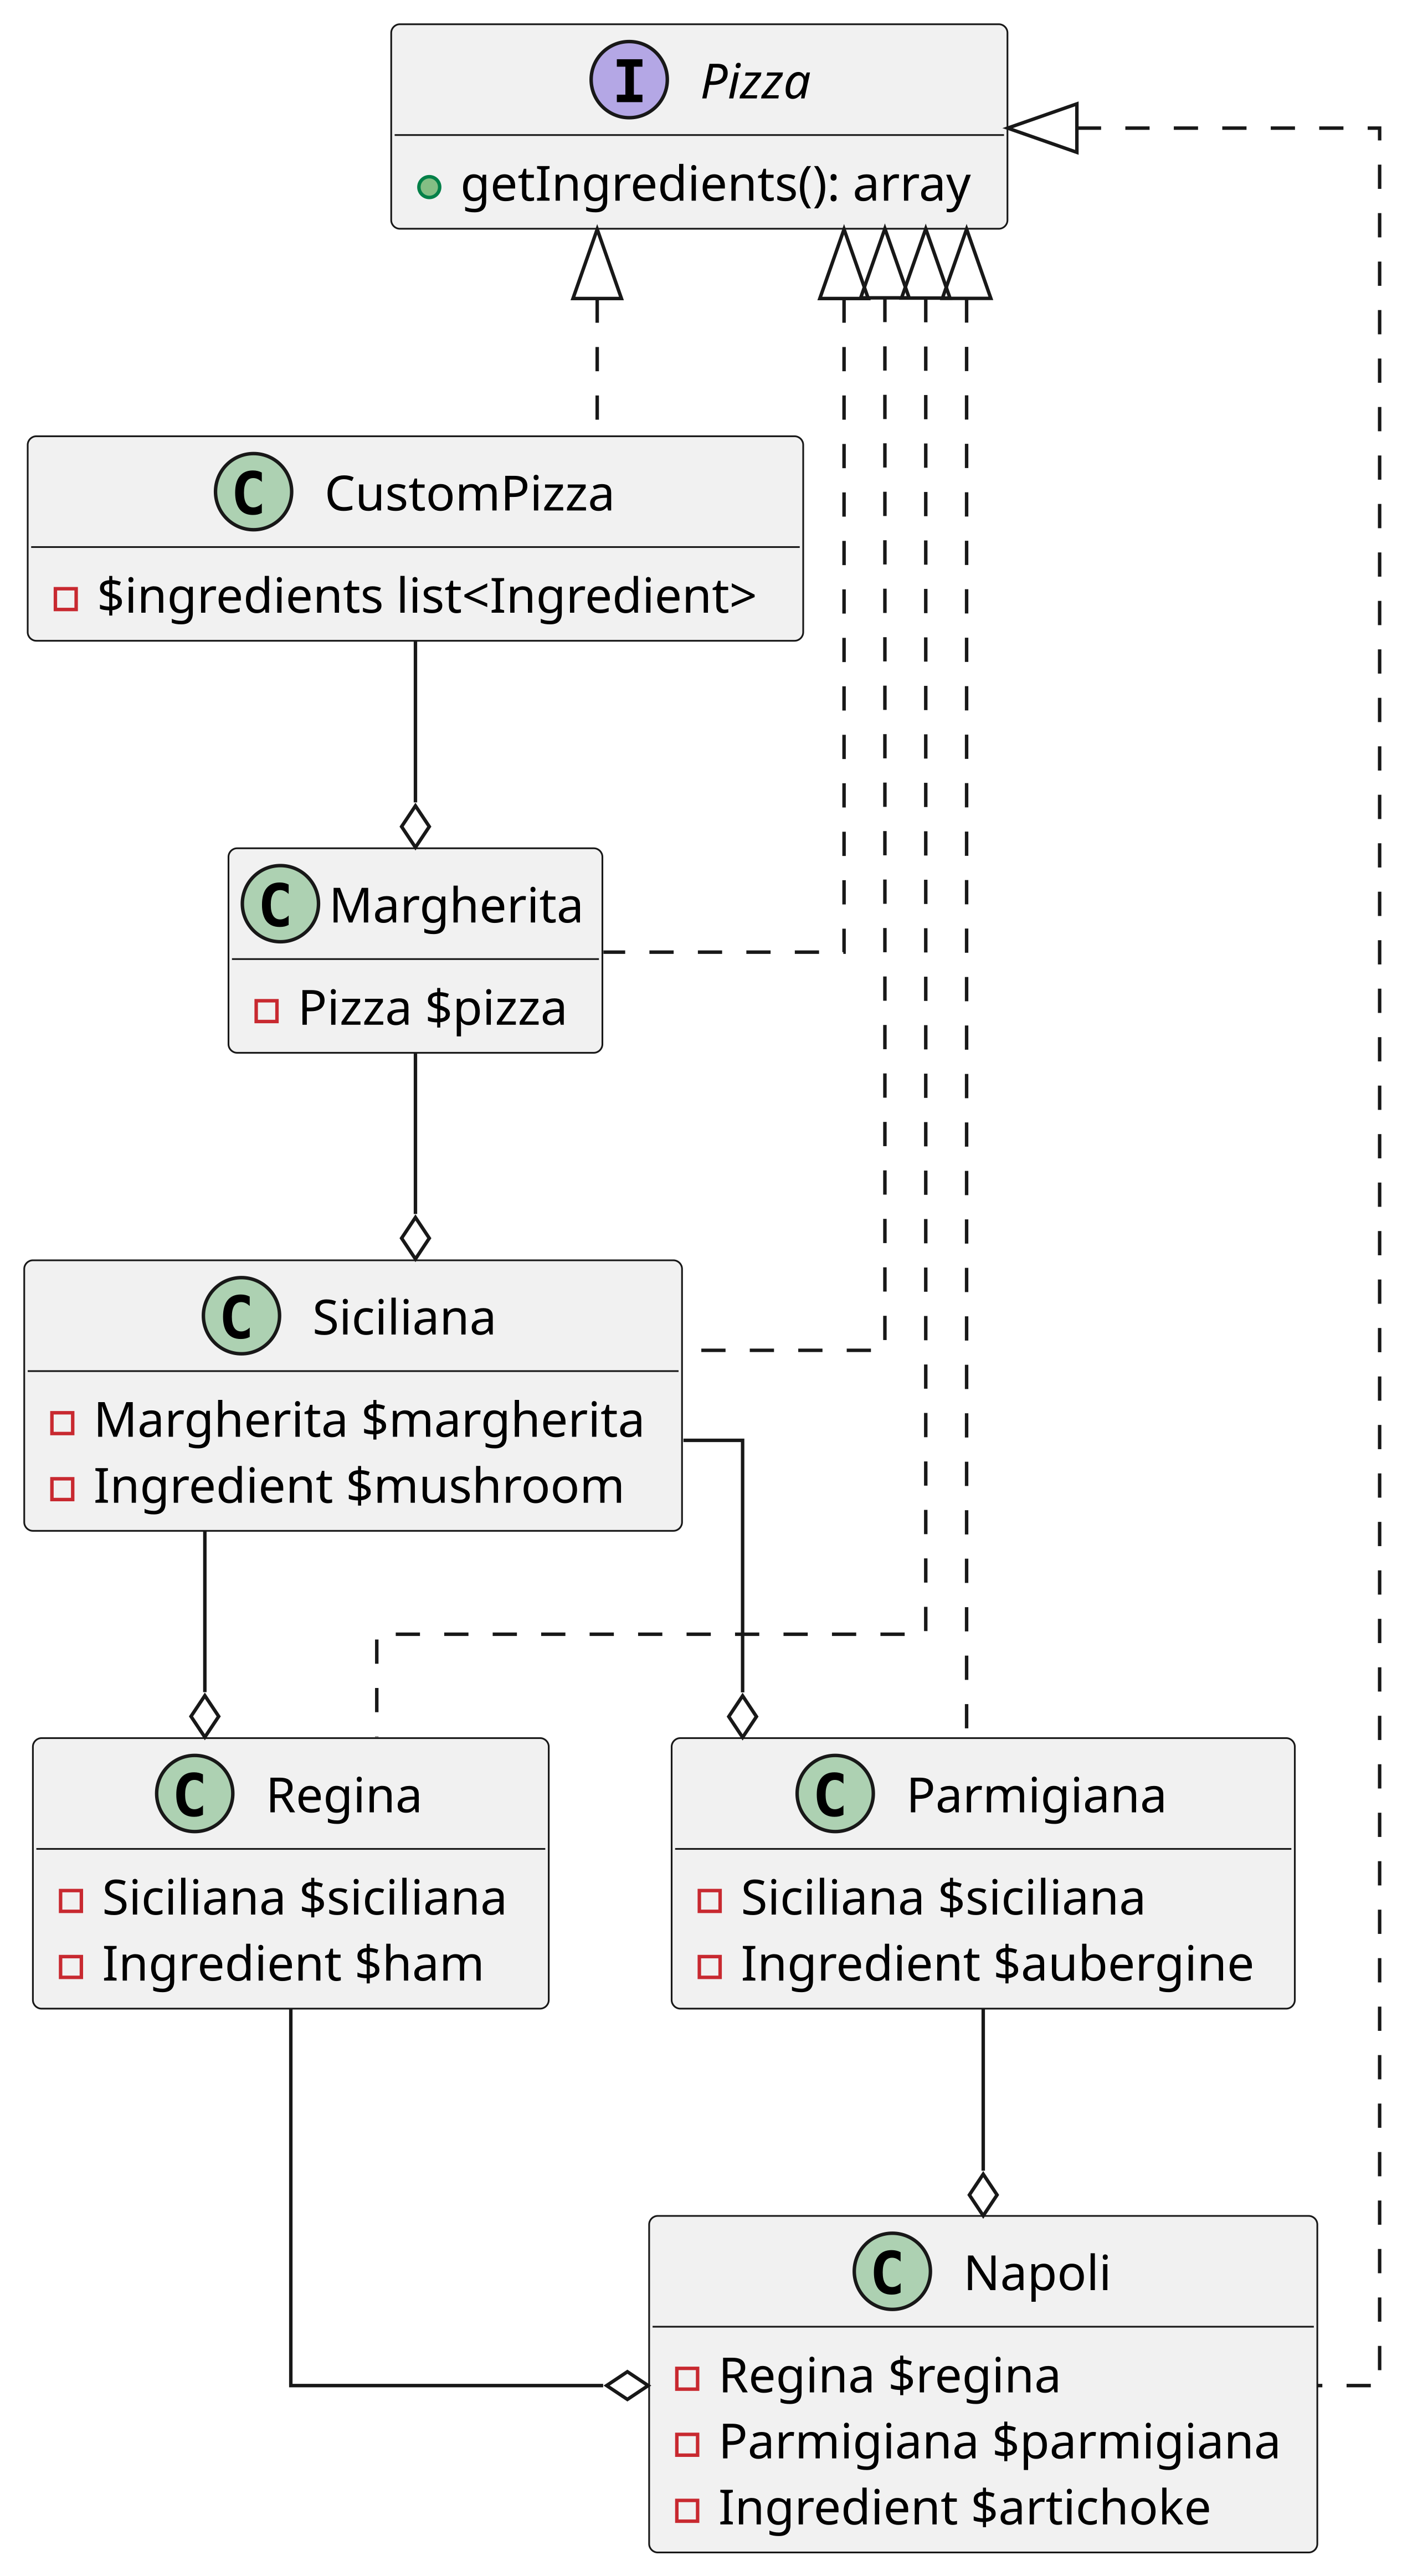
\includegraphics[height=\textheight]{src/session--composition-and-inheritance/resources/summary-composition-pizza.png}
    \end{center}
\end{frame}

\begin{frame}[fragile,c]
    \begin{lstlisting}
<?php

interface Ingredient {}

interface Pizza {
    public function getIngredients(): array;
}
    \end{lstlisting}
\end{frame}

\begin{frame}[fragile,c]
    \begin{lstlisting}
<?php

final class CustomPizza implements Pizza
{
    public function __construct(
        private Ingredient ...$ingredients
    ) {}

    public function getIngredients(): array
    {
        return $this->ingredients;
    }
}
    \end{lstlisting}
\end{frame}

\begin{frame}[fragile,c]
    \begin{lstlisting}
<?php

final class Margherita implements Pizza
{
    public function __construct(
        private Pizza $customPizza
    ) {}

    public function getIngredients(): array
    {
        return $this->customPizza->getIngredients();
    }
}
    \end{lstlisting}
\end{frame}

\begin{frame}[fragile,c]
    \begin{lstlisting}
<?php

final class Siciliana implements Pizza
{
    public function __construct(
        private Marguerita $margherita,
        private Ingredient $mushroom
    ) {}

    public function getIngredients(): array
    {
        return [...$this->margherita->getIngredients(), $this->mushroom];
    }
}
    \end{lstlisting}
\end{frame}

\begin{frame}[fragile,c]
    \begin{lstlisting}
<?php

final class Regina implements Pizza
{
    public function __construct(
        private Siciliana $siciliana,
        private Ingredient $ham
    ) {}

    public function getIngredients(): array
    {
        return [...$this->siciliana->getIngredients(), $this->ham];
    }
}
    \end{lstlisting}
\end{frame}

\begin{frame}[fragile,c]
    \begin{lstlisting}
<?php

final class Parmigiana implements Pizza
{
    public function __construct(
        private Siciliana $siciliana,
        private Ingredient $aubergine
    ) {}

    public function getIngredients(): array
    {
        return [...$this->siciliana->getIngredients(), $this->aubergine];
    }
}
    \end{lstlisting}
\end{frame}

\begin{frame}[fragile,c]
    \begin{lstlisting}
<?php

final class Napoli implements Pizza
{
    public function __construct(
        private Regina $regina,
        private Parmigiana $parmigiana,
        private Ingredient $artichoke
    ) {}

    public function getIngredients(): array
    {
        return [
            ...$this->regina->getIngredients(),
            ...$this->parmigiana->getIngredients(),
            $this->artichoke
        ];
    }
}
    \end{lstlisting}
\end{frame}

\begin{frame}[fragile,c]
    \begin{lstlisting}
<?php

var_dump($margherita instanceof Pizza);       // true
var_dump($margherita instanceof $siciliana);  // false
var_dump($margherita instanceof $regina);     // false
var_dump($margherita instanceof $parmigiana); // false
var_dump($margherita instanceof $napoli);     // false
    \end{lstlisting}
\end{frame}

\begin{frame}[fragile,c]
    \begin{lstlisting}
<?php

$tomato = new Tomato;
$cheese = new Cheese;
$mushroom = new Mushroom;
$ham = new Ham;
$aubergine = new Aubergine;
$artichoke = new Artichoke;

$basePizze = new CustomPizza($tomato, $cheese);

$margherita = new Margherita($basePizza);

$siciliana = new Siciliana($margherita, $muschroom);

$regina = new Regina($siciliana, $ham);

$parmigiana = new Parmigiana($siciliana, $aubergine);

$napoli = new Napoli($regina, $parmigiana, $artichoke);
    \end{lstlisting}
\end{frame}


\begin{frame}
    \frametitle{Object-oriented programming with composition}
    \framesubtitle{Real life example}

    \begin{itemize}[<+->]
        \item Each dependency is created,
        \item Each dependency is injected when it's needed.
    \end{itemize}
\end{frame}

\begin{frame}[fragile,c]
    \begin{lstlisting}
    <?php

    /**
     * Last-In-First-Out (LIFO) stack.
     */
    final class Stack {
        private ArrayObject $stack;

        public function __construct() {
            $this->stack = new ArrayObject;
        }

        public function push(mixed $value): void
        {
            $this->stack->append($value);
        }

        public function pop(): mixed
        {
            $arrayCopy = $this->stack->getArrayCopy();
            $result = array_pop($arrayCopy);
            $this->stack->exchangeArray($arrayCopy);

            return $result;
        }
    }
    \end{lstlisting}
\end{frame}

\begin{frame}
    \frametitle{Object-oriented programming with composition}
    \framesubtitle{Key points}

    \begin{itemize}[<+->]
        \item No \texttt{extends} needed,
        \item Internals are hidden from public interface,
        \item Internals are \textit{swap-able} without altering the public interface,
        \item The \texttt{final} keyword enforces the \texttt{Composition} pattern.
    \end{itemize}
\end{frame}

\begin{frame}
    \frametitle{Object-oriented programming with composition}
    \framesubtitle{Issues}

    \begin{itemize}[<+->]
        \item No \textit{Yo-Yo} problem
        \item No hard relation between a class and another
        \item No inheritance of unnecessary methods
        \item No flexibility issue as a class is not supposed to extend another
        \item No \texttt{is-a} relation, now replaced with \texttt{has-a}.
    \end{itemize}
\end{frame}

\begin{frame}[fragile,c]
    \begin{center}
        
\includegraphics[height=\textheight]{src/session--composition-and-inheritance/meme/feels-good.png}
    \end{center}
\end{frame}

\begin{frame}
    \begin{quote}
        Simplicity is the ultimate sophistication.\\~\\

        \hfill Leonardo Da Vinci
    \end{quote}
\end{frame}

\begin{frame}
    \begin{quote}
        But wait\ldots \pause I'm pretty sure I already saw that somewhere!
    \end{quote}
\end{frame}

\begin{frame}[fragile,c]
    \noindent\begin{minipage}{.45\textwidth}
        \begin{center}
            \large{Composition}
            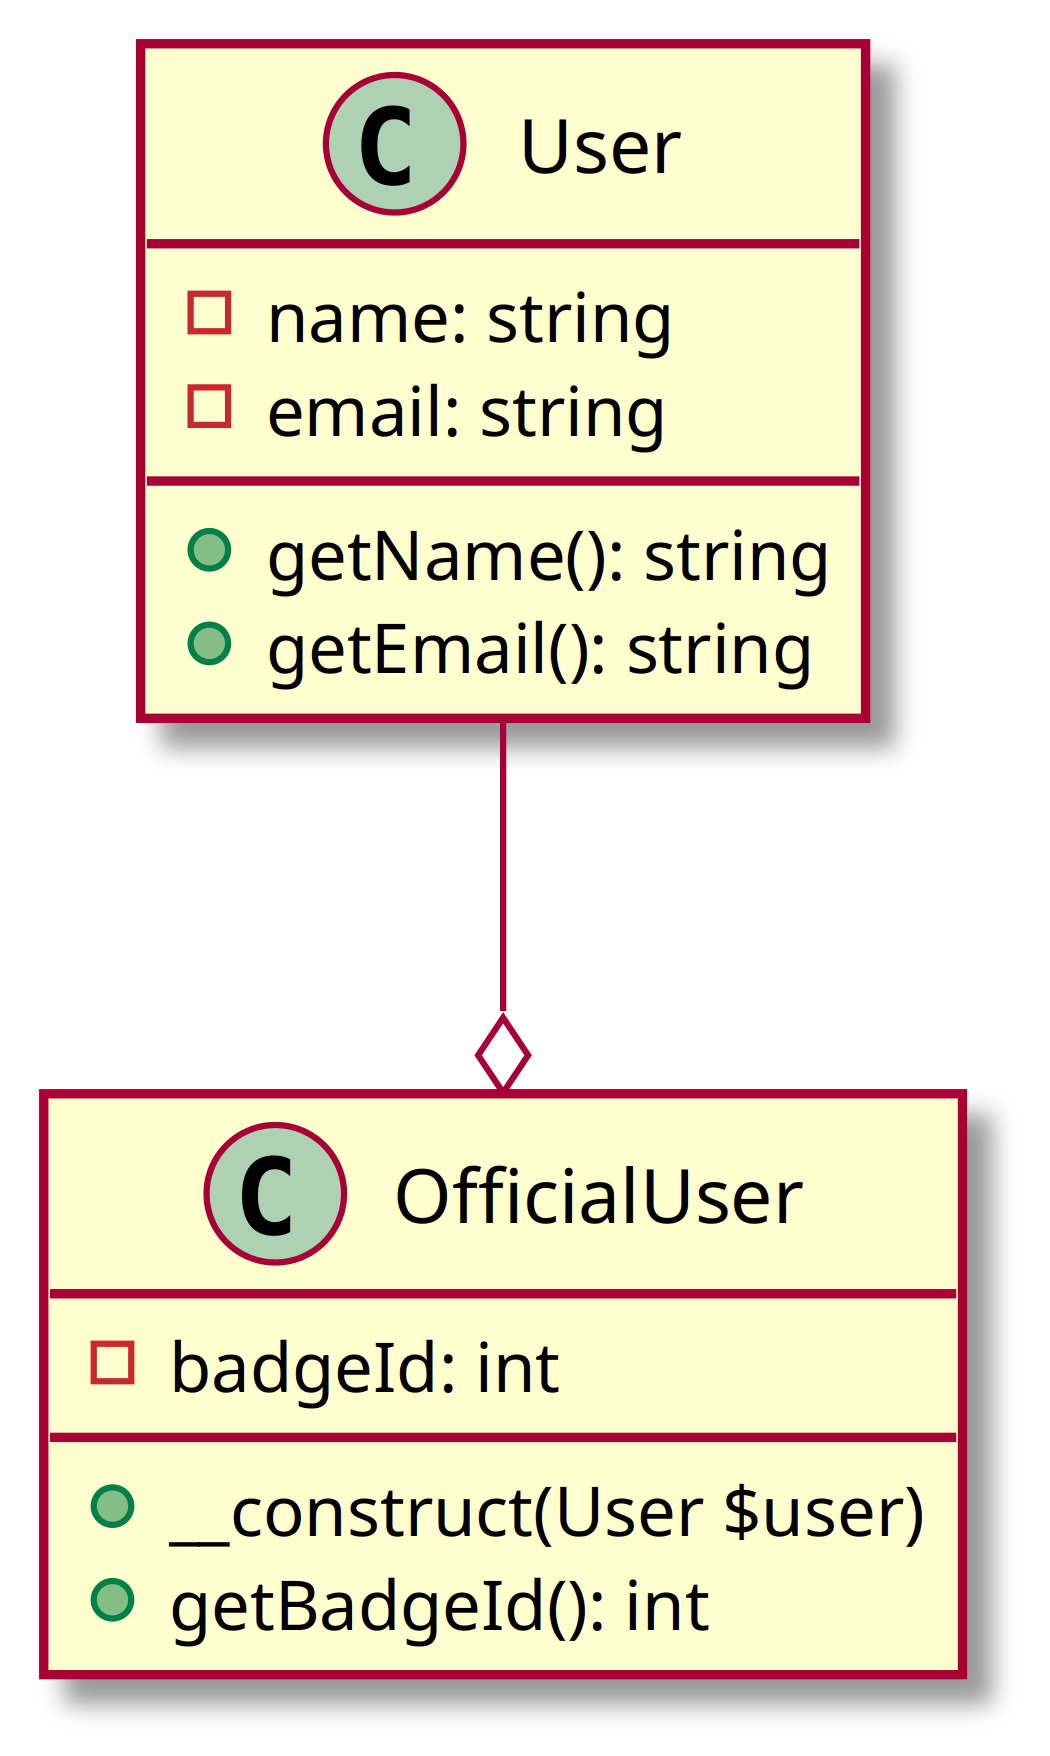
\includegraphics[height=.75\textheight]{src/session--composition-and-inheritance/resources/Composition.png}
        \end{center}
    \end{minipage}\hfill
    \begin{minipage}{.10\textwidth}
        \pause
    \end{minipage}
    \begin{minipage}{.45\textwidth}
        \begin{center}
            \large{Inheritance}
            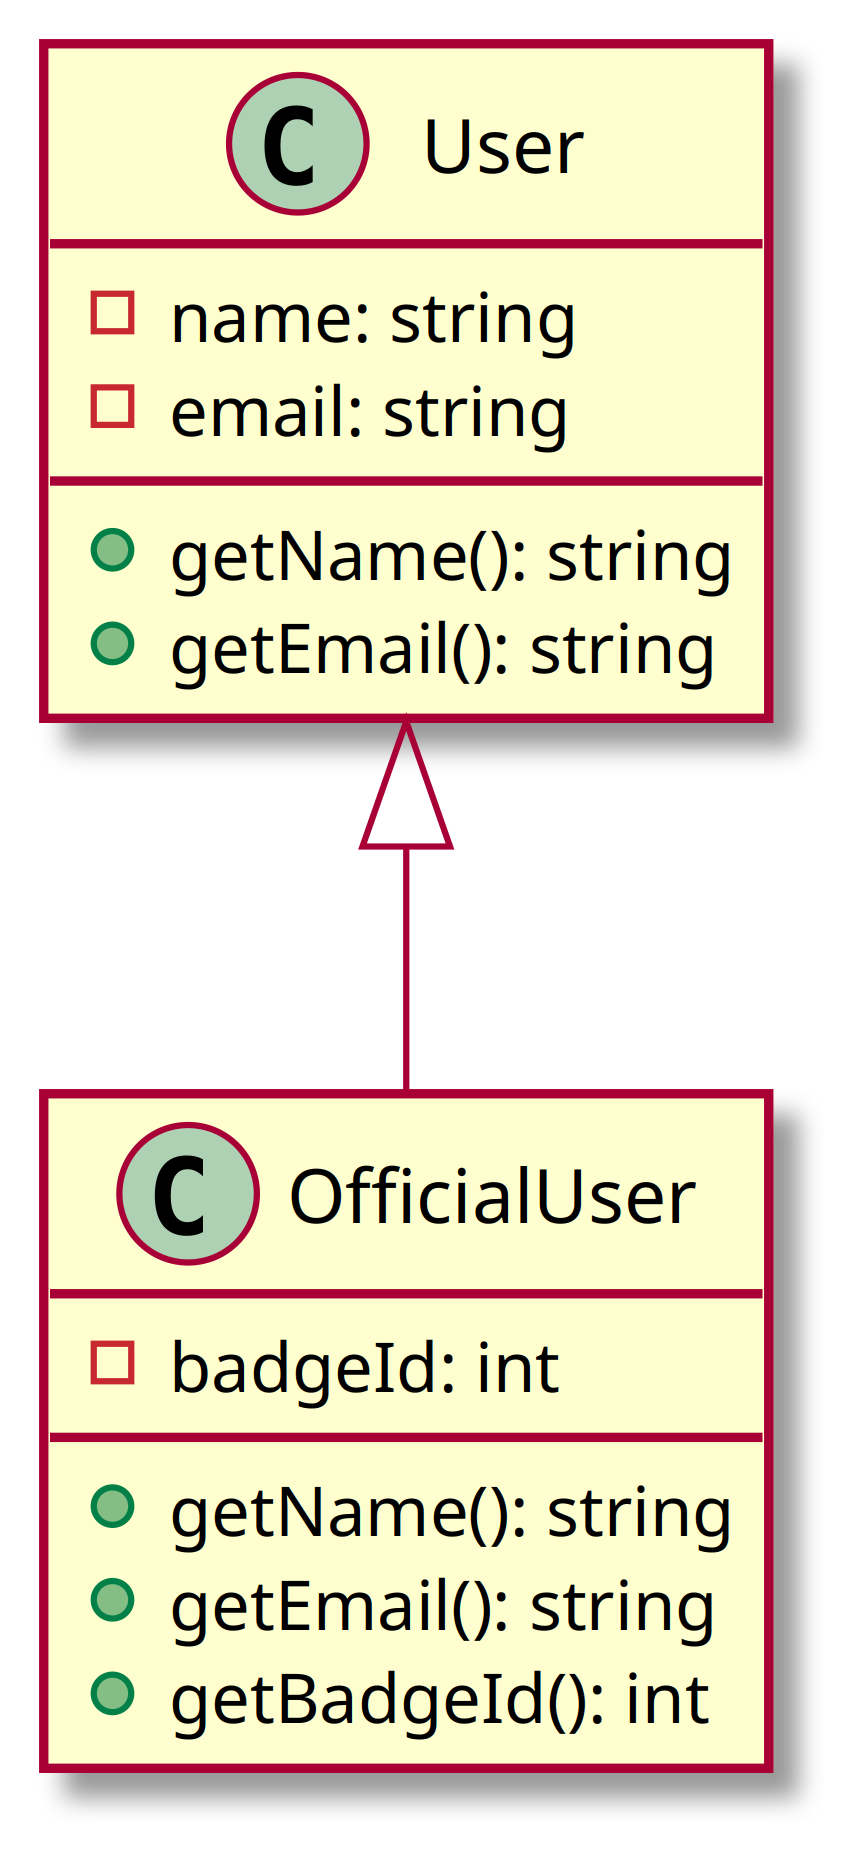
\includegraphics[height=.75\textheight]{src/session--composition-and-inheritance/resources/Inheritance.png}
        \end{center}
    \end{minipage}
\end{frame}

\begin{frame}[fragile,c]
    \begin{center}
        \large{Decorator pattern}
        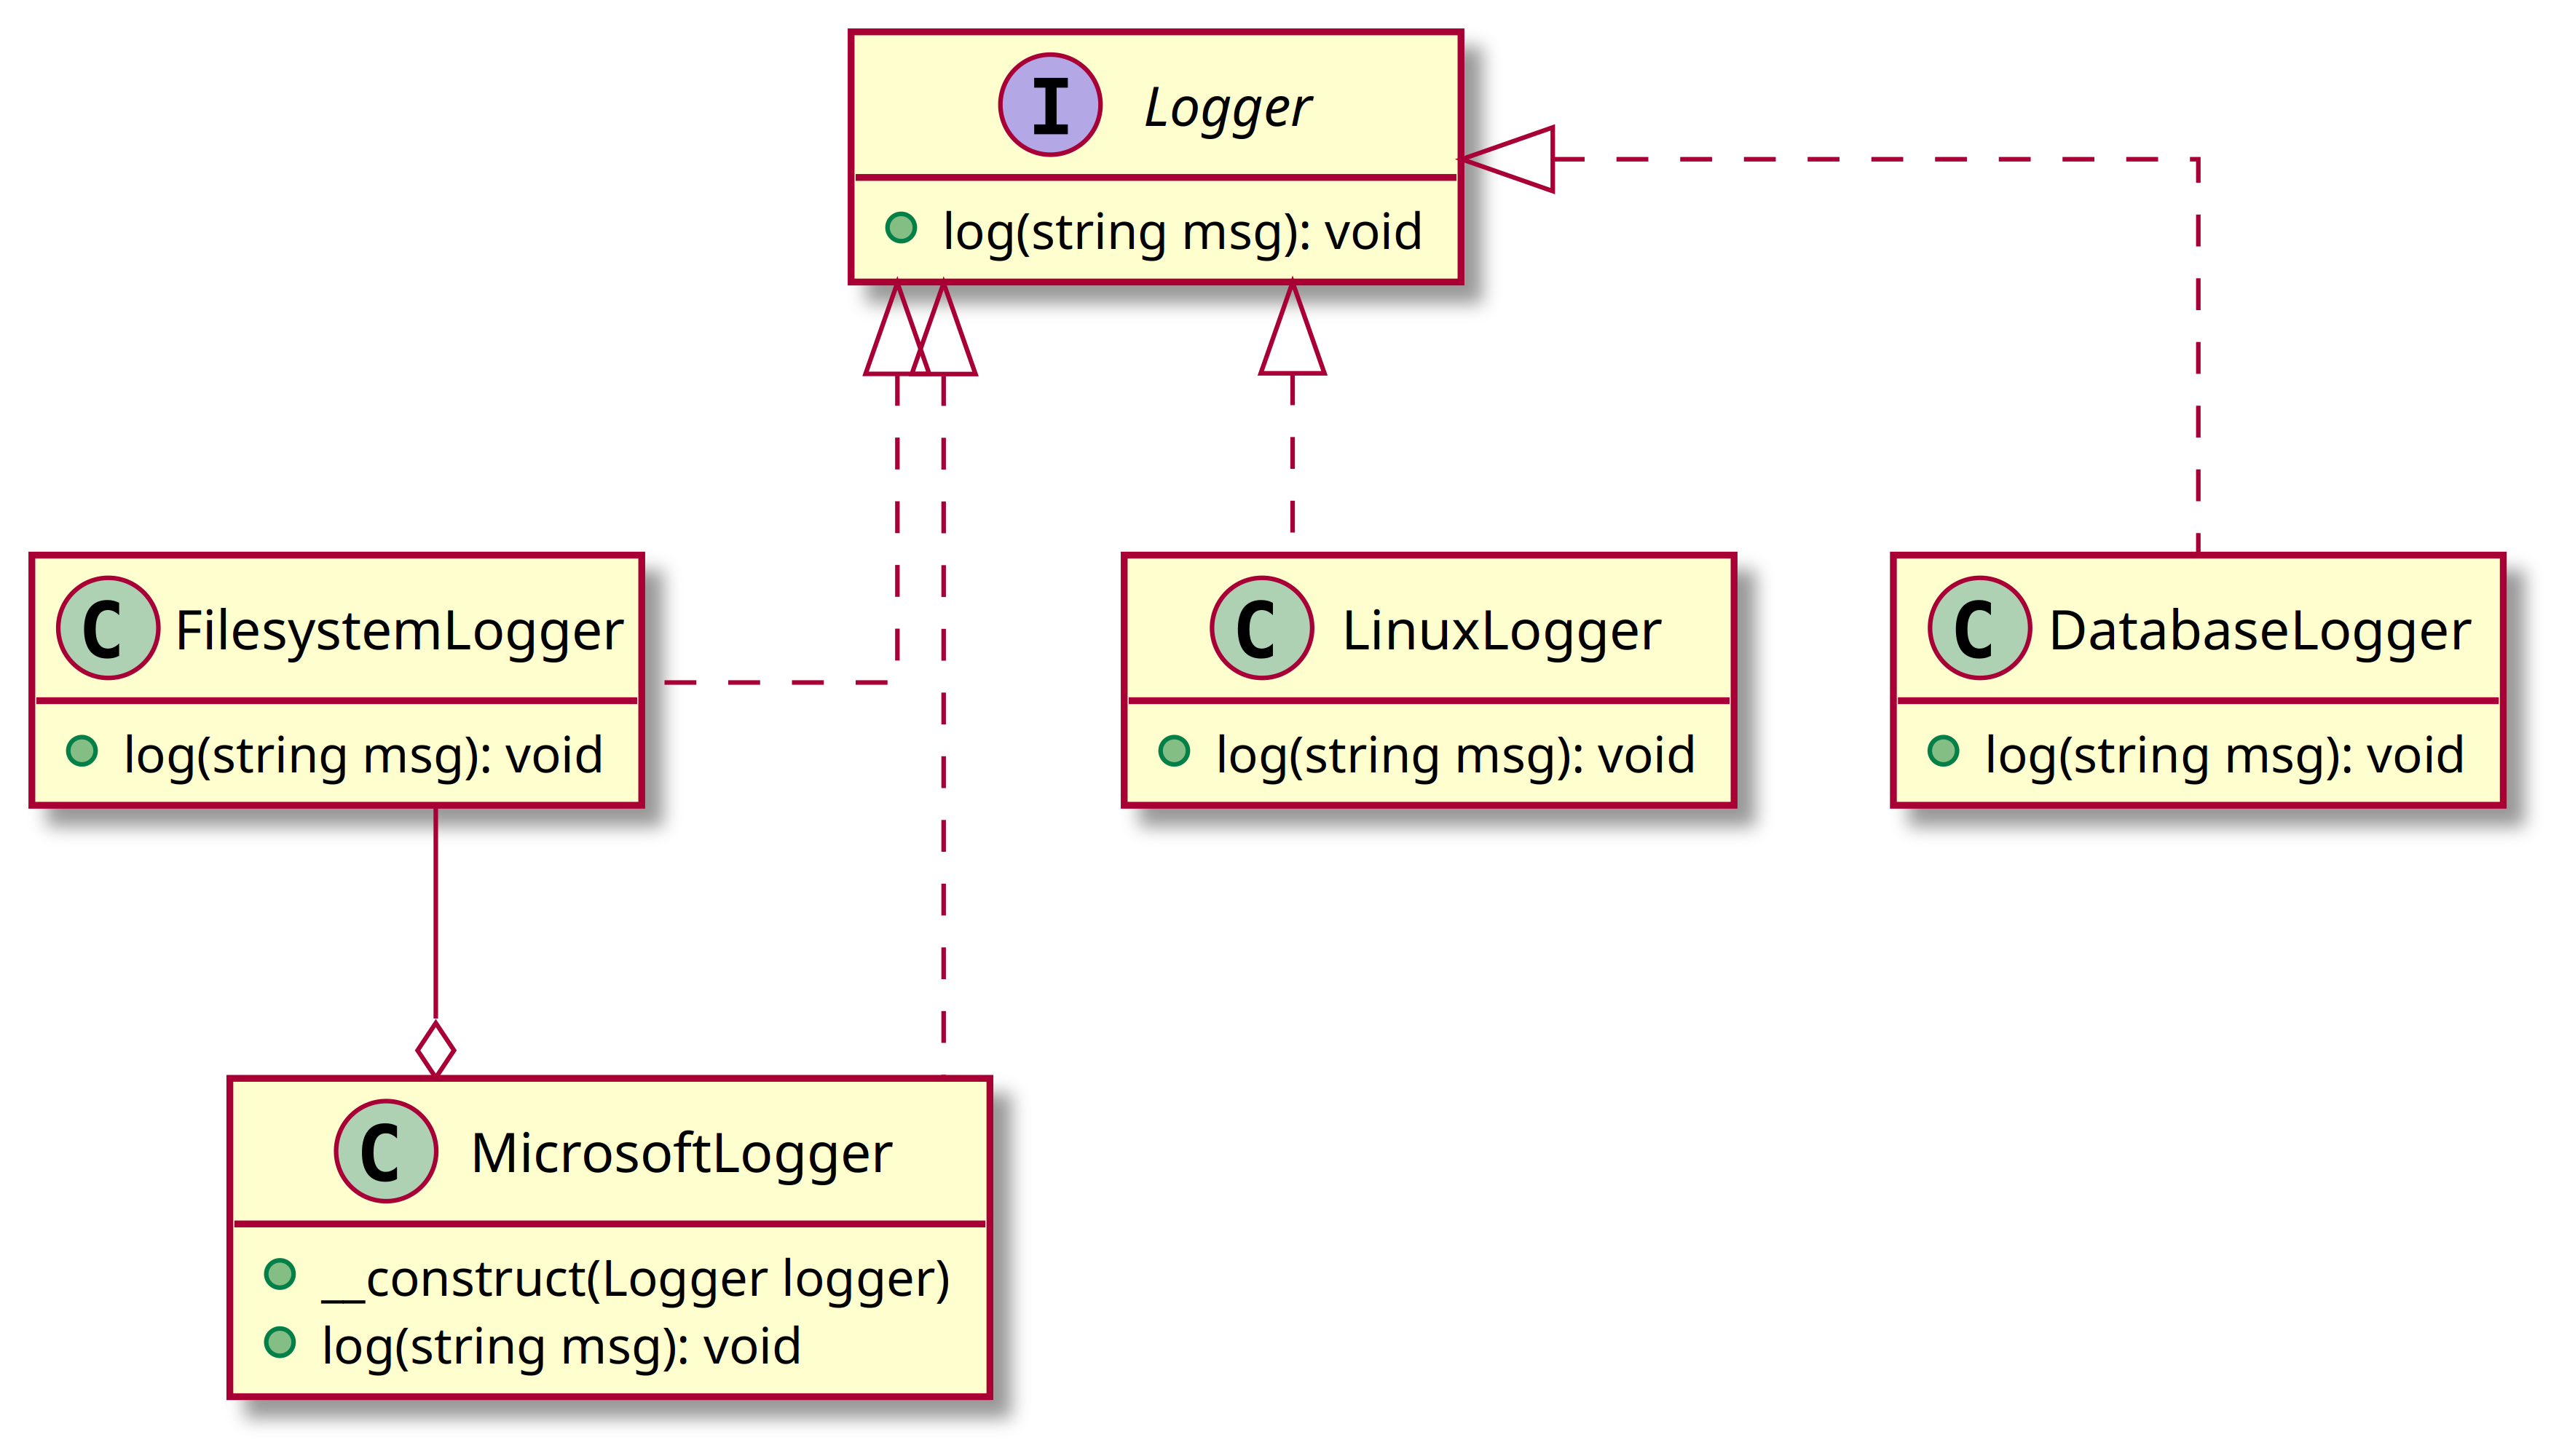
\includegraphics[width=\textwidth]{src/session--composition-and-inheritance/resources/decorator-pattern.png}
    \end{center}
\end{frame}

